\documentclass{report}
\usepackage[T1]{fontenc}
\usepackage[utf8]{inputenc}
\usepackage[francais]{babel}
\usepackage{graphicx}
\usepackage[hidelinks]{hyperref}
\usepackage{url}
\usepackage{rotating}

\title{Cahier des charges~: \\Projet Développement d'un dot-plot en HTML, JavaScript et WebGL }
\author{Rania \bsc{Assab} \\ Aurélien \bsc{Luciani}\\ Quentin \bsc{Riché-Piotaix}\\ Mathieu \bsc{Schaeffer}}
\date{5 mars 2014}
\begin{document}

\maketitle

\tableofcontents
\addcontentsline{toc}{chapter}{Introduction}
\chapter*{Introduction}

Le dot-plot est une manière de comparer des séquences ---~nucléotidiques ou protéiques~--- pour mettre en évidence les séquences répétées ou palindromiques. C'est une technique remontant aux années 70 mais elle demeure efficace pour en avoir une vue générale.\\
Les éléments sont comparés deux à deux et les résultats de la comparaison sont illustrés par un graphique qui permet de mettre en évidence des zones d'intérêt.\\
De par la nature du dot-plot, la comparaison ne peut être effectuée qu'entre séquences de même type.\\
L'objectif du projet est d'implémenter une application utilisant les technologies web actuelles, ne nécessitant aucune extension navigateur et produisant le même type de résultat.

\chapter{Fonctionnement du dot-plot}

Pour pouvoir interpréter les résultats, il faut comprendre comment se déroule le processus de comparaison. Par exemple, dans le cas de deux séquences de nucléotides~: La première base de la première séquence est comparée avec la première base de la seconde séquence. Une matrice d'alignement de séquence doit être choisie pour l'analyse.\\
Son choix est important car selon la matrice choisie, le résultat sera différent. Les matrices doivent être sélectionnées selon les séquences à analyser car il en existe avec des pondérations différentes donnant des scores différents.\\
Pour représenter ceux-ci de manière ergonomique, à chaque score est associé une couleur dans un gradient, permettant de visualiser des motifs, comme des diagonales (cf fig.\ref{schema}). On peut alors en déduire la présence de similitudes ou de palindromes dans les séquences.\\

\begin{figure}[!ht]
\centerline{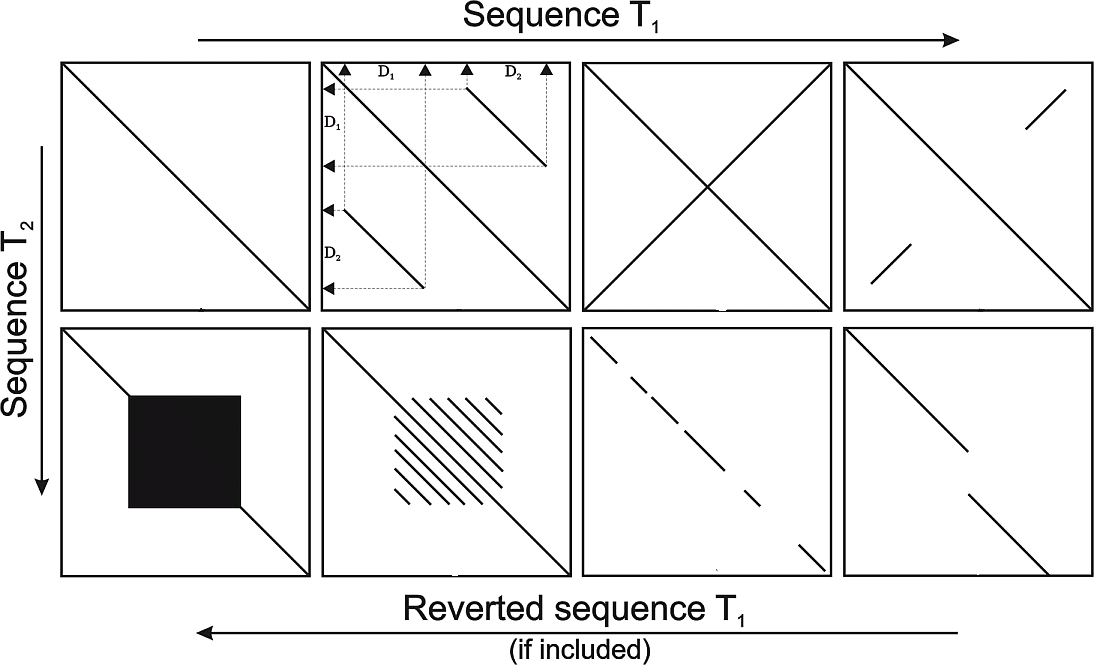
\includegraphics[scale=0.45]{SchemaDotplot.png}}
\caption{Représentation de différents résultats (\bsc{Schulz}, \bsc{Leese} et \bsc{Held}, 2008)}
\label{schema}
\end{figure}

\chapter{Dotlet}
\section{Historique}
Dotlet est une application disponible en ligne permettant de comparer deux séquences nucléotidiques ou protéiques en se basant sur la méthode du dot-plot. Cependant, pour pouvoir l'utiliser, il faut que la machine virtuelle Java soit installée sur la machine et disponible dans le navigateur.\\
Ce logiciel a été codé par Marco Pagni et Thomas Junier, du Swiss Institute of Bioinformatics à Épalinges en Suisse. Jusqu'à présent, il n'y avait pas d'application permettant la comparaison de séquences à travers un navigateur web. Ils ont alors pris l'initiative de la faire et ont même continué son développement. En effet, la version 1.5 est sortie récemment avec plus de fonctionnalités.

\section{Utilisation}

L'interface graphique (cf fig \ref{dotletInterface}) permet la saisie des deux séquences à comparer. Elle s'effectue via un copier-coller. Il est nécessaire de choisir une matrice d'alignement~: Identité (par défaut), BLOSUM \footnote{\emph{BLOcks SUbstitution Matrix}}, PAM \footnote{\emph{Point Accepted Mutation}}, etc. Il est aussi possible de choisir une taille de fenêtre de comparaison et un zoom particuliers.\\
Les comparaisons peuvent se faire entre deux séquences d'ADN, deux protéines ou entre une séquence d'ADN et une séquence protéique. Dans ce dernier cas, l'ADN est traduit en séquence protéique par le biais des différents cadres de lecture possibles.\\

\begin{figure}[!ht]
\centerline{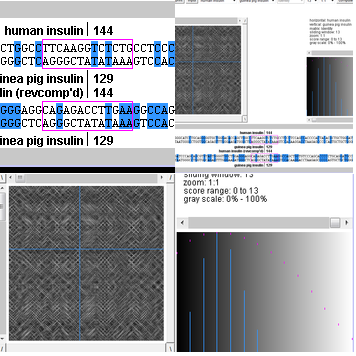
\includegraphics[scale=0.75]{dotlet.png}}
\caption{Différentes vues de l'interface actuelle de Dotlet}
\label{dotletInterface}
\end{figure}

\chapter{Exigences}
\section{Besoins fonctionnels}
Selon les exigences données, il va falloir se conformer au Dotlet précédemment décrit.\\
Cet outil ayant été validé et utilisé pendant une dizaine d'années par de nombreux scientifiques, professeurs et étudiants, il représentera donc la référence.\\
L'objectif est d'en réaliser une version web plus accessible, utilisant les technologies HTML (\cite{html5}), WebGL (\cite{khronos}) et JavaScript (\cite{javascript}). Celles-ci ayant évolué, il est maintenant possible de le faire sans utiliser Java et de ne plus dépendre d'un module externe.

\paragraph{Web} ~\\
Cet outil de dot-plot devra être disponible directement sur le web, cependant, le code devra être compatible avec les principaux navigateurs du marché.
Dans un premier temps, seuls les navigateurs Chrome et Firefox sont demandés.

\paragraph{Menu} ~\\
Tout d'abord, il va falloir réaliser un menu permettant d'initialiser les différents paramètres de ce dot-plot, incluant~:
\begin{itemize}
	\item L'enregistrement de séquences a comparer, via une entrée de texte.
	\item Le choix des deux séquences dans une liste déroulante, parmi les séquences enregistrées.
	\item Le choix de la matrice de comparaison parmi celles récupérés dans la littérature.
	\item La taille de la fenêtre de comparaison, pour plus ou moins de précision dans notre dot-plot.
\end{itemize}

\paragraph{Graphe} ~\\
	L'affichage des résultats se fera sur un graphe traduisant les scores obtenus entre les deux séquences, représentées en abscisse et en ordonnée. Ceux-ci sont représentés par un gradient de couleurs.\\
Chaque pixel de l'image représentera donc le score calculé selon la matrice et la taille de la fenêtre de comparaison passées en paramètres.

\paragraph{Fenêtre d'alignement} ~\\
	Une vision plus précise sera donnée par l'affichage d'une fenêtre d'alignement entre les deux séquences.
Des ascenseurs permettront de naviguer sur celles-ci et de choisir une position pour chacune d'entre elle.\\
Devront y figurer la fenêtre de comparaison ainsi que le degré de similitude entre les éléments comparés.\\
D'autre part, certains cas particuliers devront être pris en compte.
Dans le cas où l'on étudierait le rapprochement entre une séquence d'ADN et une protéine, l'alignement comprendra la séquence protéique initiale, ainsi que les trois séquences protéiques traduites des trois cadres de lectures de la séquence nucléotidique.
Pour une comparaison entre ADN, les séquences seront comparées dans le même sens et dans des sens opposés.\\
Un clic sur l'image capturera les positions des séquences et l'alignement s'initialisera à partir de celles ci.

\paragraph{Histogramme} ~\\
L'histogramme correspondant au graphique sera ajouté, de plus il fera apparaître les valeurs logarithmiques pour distinguer les plus petites variations.
Des ascenseurs permettront de faire fluctuer le contraste et de se focaliser uniquement sur certaines valeurs. Ces modifications  se répercuteront sur l'image, permettant de révéler des diagonales intéressantes pour notre analyse.

\section{Besoins non fonctionnels}

\subsection{Fonctionnalités de la version 1.5}
Certaines fonctionnalités qui ne sont pas essentielles au bon déroulement de l'application ont été implémentées avec la version 1.5 du logiciel. Il s'agit notamment de l'ajout d'un bouton permettant d'imprimer le graphique affiché. Cette fonctionnalité pourra être remplacée par la possibilité de récupérer l'image.\\
Les autres ajouts permettent, en combinant une action de la souris et une touche du clavier, de sélectionner des zones d'intérêt dans l'image. Cela peut être une diagonale contenue dans la zone choisie si au moins la moitié des valeurs des points de cette diagonale dépasse un certain seuil, défini par l'utilisateur. Les séquences de ces diagonales peuvent ensuite être récupérées au format FASTA.\\
C'est également le cas pour une autre fonctionnalité~: l'utilisateur peut, en cliquant sur un point, récupérer la séquence de la diagonale sur laquelle il a cliqué, tant que les valeurs de cette diagonale sont au dessus du seuil qu'il a défini. Quand cette action est répétée, les séquences s'ajoutent.\\
Enfin, le dernier ajout, appelé «~curseur magnétique~» permet de voir facilement le positionnement dans les séquences avec un simple survol de la zone d'intérêt.

\subsection{Amélioration de certains points}
Quelques aspects de l'application Dotlet ne sont pas très satisfaisants ou ergonomiques et pourraient être améliorés pour donner plus de confort et de rigueur à l'utilisateur.\\
Pour ce qui est du zoom, la façon de faire est peu intuitive, et il serait préférable d'utiliser la molette de la souris. L'autre point important est la gestion de la traduction. En effet, on peut choisir de comparer une séquence nucléotidique avec une séquence protéique, mais en raison des multiples cadres de lecture lors de la traduction, le meilleur score issu des trois comparaisons pour chaque acide aminé sera alors affiché. Une solution pourrait être de distinguer les trois cadres de lecture lors de l'affichage. Enfin, l'interface pourrait gagner en esthétisme et en ergonomie.

\section{Test du programme}

Des jeux de données seront utilisés pour s'assurer de la validité des résultats. Ils permettront de comparer les résultats issus du Dotlet avec ceux issus du projet.
Les séquences utilisées seront celles de la doc de Dotlet~:
\begin{itemize}
	\item Protéine de SLIT \emph{Drosophila melanogaster} (P24014) contre elle-même.
	\item Antigène membranaire MS2 humain (P78325) contre Adamalysine II de \emph{Crotalus adamanteus} (P34179).
	\item Le gène codant pour la calmoduline (J05545) contre la protéine résultante (P19533) chez l'\emph{Emericella nidulans}.
	\item Le gène codant pour la UTP-glucose-1-phosphate uridylyltransferase de \emph{Bacillus subtilis} (L12272) contre lui-même.
	\item Le précurseur du récepteur au facteur de stimulation de colonie de granulocytes de \emph{Mus musculus} (P40223) contre un gène codant pour une protéine non-identifiée.
\end{itemize}

\chapter{Environnement de programmation}

Dans le cadre de ce projet, plusieurs langages seront utilisés. Les langages HTML5 et CSS3 (\cite{css3}) serviront à structurer l'affichage dans les navigateurs web.\\
Contrairement à Dotlet, le cœur de l'application se fera en JavaScript, un langage de programmation de scripts offrant l'interactivité nécessaire à l'application. De plus, cela permettra d'effectuer les calculs chez l'utilisateur et non sur un serveur distant.\\
JavaScript est aussi nécessaire pour utiliser la technologie WebGL, une interface de programmation permettant d'accéder depuis le navigateur à la technologie OpenGL \footnote{\emph{Open Graphics Library for Embedded System}}. Cette dernière est une bibliothèque graphique utilisant les ressources de la carte graphique.
La partie en WebGL permettra d'optimiser certains calculs en les effectuant sur la carte graphique et d'accélérer ainsi l'affichage du résultat.\\
Pour le développement, le système de gestion de version décentralisé Git sera utilisé, en particulier grâce aux services offerts par GitHub (\cite{github}).

\chapter{Interface}
L'interface de l'application suivra les grandes lignes de Dotlet avec quelques modifications permises par l'amélioration des technologies web. La structure sera découpée en zones logiques qui sépareront et simplifieront les différentes étapes de l'analyse. En premier se situeront les réglages pré-traitement, suivis de l'affichage des résultats et enfin des outils pour affiner l'analyse (cf fig. \ref{maquette}).\\

\begin{figure}[!ht]
\centerline{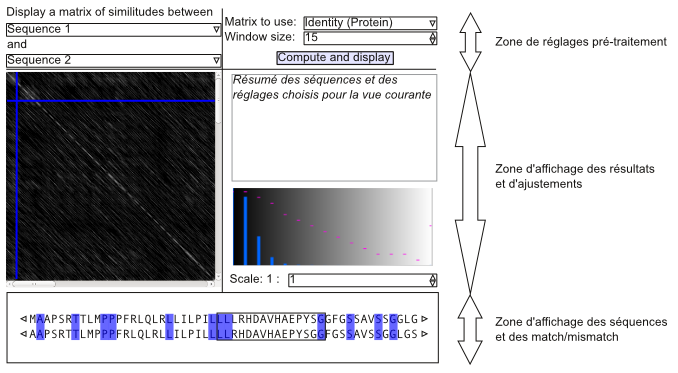
\includegraphics[scale=0.60]{maquette.png}}
\caption{Maquette}
\label{maquette}
\end{figure}

\begin{sidewaysfigure}
\chapter{Planning prévisionnel}
\centerline{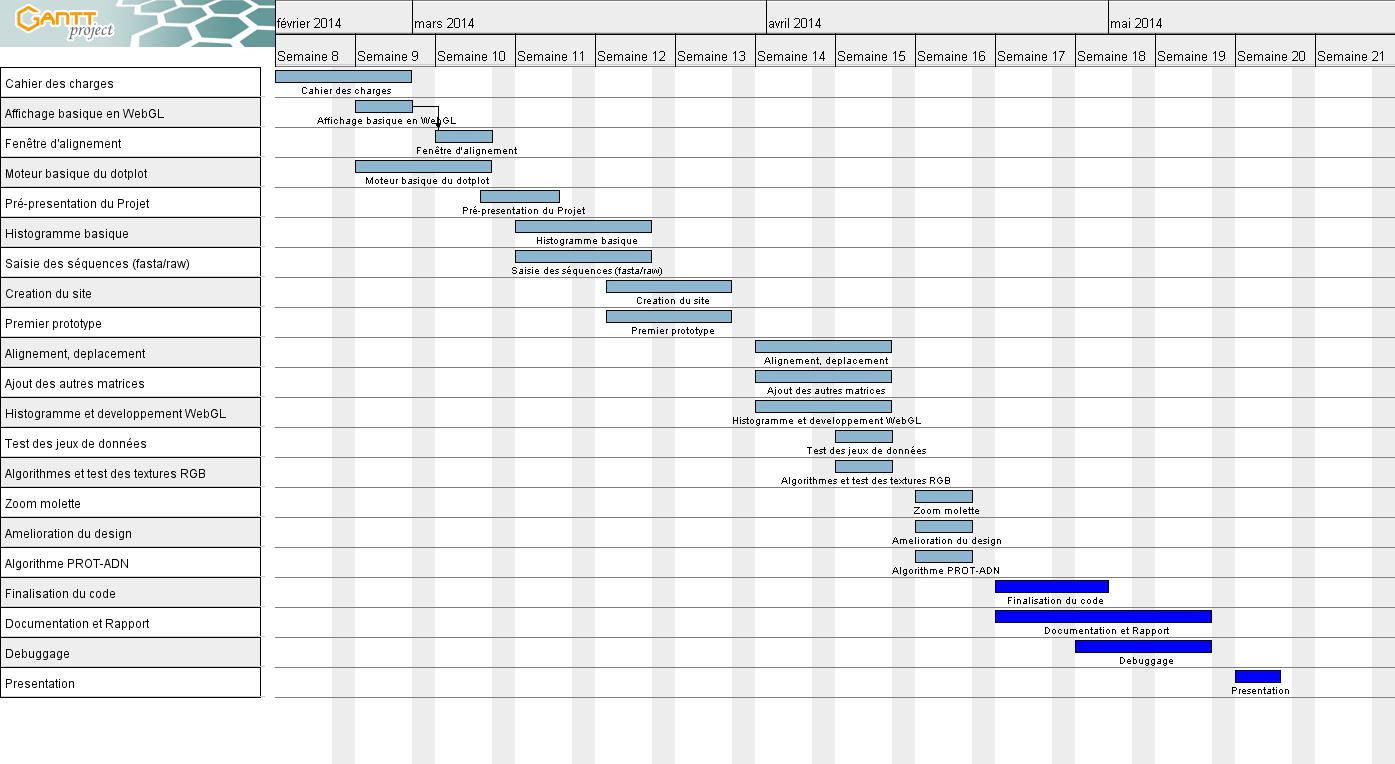
\includegraphics[scale=0.55]{planning.png}}
\caption{planning}
\end{sidewaysfigure}

\begin{thebibliography}{9}
\addcontentsline{toc}{chapter}{Bibliographie}
\bibitem{dotlet}
  \emph{Site web de Dotlet}.
  \url{http://myhits.isb-sib.ch/cgi-bin/dotlet}
\bibitem{SIB}
  \emph{Site web du Swiss Institute of Bioinformatics}.
  \url{https://www.isb-sib.ch/}
\bibitem{articleDotlet}
  Thomas \bsc{Junier}, Marco \bsc{Pagni},
  \emph{Dotlet: diagonal plots in a Web browser},
  2000. Oxford University Press.
  \url{http://bioinformatics.oxfordjournals.org/content/16/2/178.long}
\bibitem{dotplot1}
  Jan \bsc{Schulz}, Florian \bsc{Leese}, Christoph \bsc{Held},
  \emph{Introduction to dot-plots},
  2008.
  \url{http://www.code10.info/index.php?view=article&id=64}
\bibitem{dotplot2}
  Jan \bsc{Schulz},
  \emph{Identity dot-plots},
  2008.
  \url{http://www.code10.info/index.php?view=article&id=69}
\bibitem{dotplot3}
  Jan \bsc{Schulz},
  \emph{Complete dot-plots},
  2008.
  \url{http://www.code10.info/index.php?view=article&id=74}
\bibitem{khronos}
  \emph{OpenGL ES 2.0 for the Web},
  \url{https://www.khronos.org/webgl/}
\bibitem{html5}
  \emph{Spécification de HTML5 par le W3C},
  \url{http://www.w3.org/TR/html5/}
\bibitem{css3}
  \emph{Spécification de CSS3 par le W3C},
  \url{http://www.w3.org/Style/CSS/current-work}
\bibitem{javascript}
  \emph{Documentation sur JavaScript par Mozilla},
  \url{https://developer.mozilla.org/fr/docs/JavaScript}
\bibitem{github}
  \emph{Site web de GitHub}.
  \url{https://github.com}
\end{thebibliography}

\end{document}
